\chapter{Methods}
In order to compare the effects of using design patterns as stated before an application is being developed. This section describes the requirements of the program in detail and presents how the two versions are being implemented.

\section{Domain Description}
The application provides a time-tracking solution for small businesses. The basic work-flow includes users (members), projects, project phases, project members and activities. A diagram of this can be seen in figure \ref{fig:data-diagram}.

\begin{itemize}
	\item \textbf{User}: A user is considered employee of the firm. She can participate in existing projects or create new projects on her own.
	\item \textbf{Project}: A project is the overall term for a distinguishable amount of work that is done for a specific customer. A project has one or more project leaders and zero or more project members.
	\item \textbf{Project Phase}: Each project exists of one or more phases that are used to monitor the progress of the project. Project leaders are able to create, adopt and delete phases for their projects. 
	\item \textbf{Project Member}: A user is considered project member of a specific project as soon he participates or leads it. Two roles exist, he can either be leader or member. A project leader has the responsibility of maintaining project specific data, such as description, phases and assigning project members. He is \emph{not} allowed to create new users. After creating a new project, one is automatically project leader. A project leader is allowed to monitor the statistics of his projects including the workloads of the project members. As a simple member one is allowed to add, delete and modify activities created by the user and is only allowed to perform this actions for projects he is assigned to. He is also only allowed to monitor his own statistics for projects he participates.
	\item \textbf{Activity}: A activity represents a workload that is done by a specific member in a specific phase for a specific project.
\end{itemize}

\begin{figure}
	\centering
	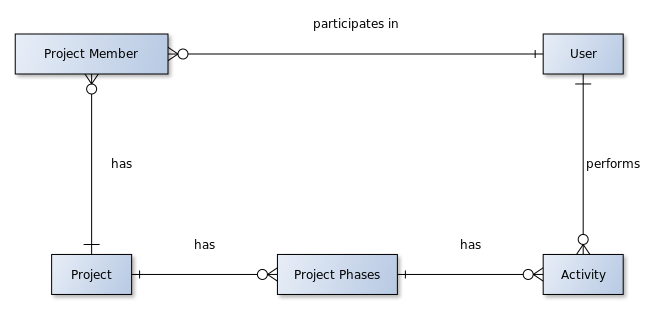
\includegraphics[width=\textwidth]{./content/pictures/data-diagram.jpg}
	\caption[Diagram of data-class relations.]{Diagram of data-class relations.}
	\label{fig:data-diagram}
\end{figure}

\subsubsection{Use-Cases}
To specify in depth how the program should work the following use-cases are set.
\begin{enumerate}
\item \textbf{Login:} After starting the program, a login prompt shall show up. The user provides his credentials which will be compared to the saved credentials in the database. If they are correct, he is forwarded to the main program. New users can register by clicking on a button in the login-view by providing his personal data and a password. A nickname needs to be picked that is not already used by another user. After successful registration the user is able to login without further action.

\item \textbf{Starting / Stopping activities:} A banner at the top of the applications main view provides means to add new activities. In order to do so the user picks one of his associated projects from a drop down menu. After selecting one a second drop down menu is populated with the available project phases. After selecting a belonging project phase he is able to click the start button. After starting a timer indicates the current time spent in the chosen phase for the activity. After clicking the stop button a input mask should pop up for the user to provide additional information of the activity he just finished, namely the description and (optional) some comments. Then the timer is reset and a new activity can be started. 

\item \textbf{Personal statistics:} Utilizing the associated button of the left side bar the main panel lists all project the user is assigned to and the time he spent working for these projects. At the top of the main panel he can choose the period he wants to see, for instance it should be possible to filter the projects for activities created in the last month. To review a specific project in detail after a double-click onto one of the project-entries all phases of the project should be listed, again with the time spent in each phase. The filtering of a specific period should be possible too. By double-clicking at a phase all activities by the user in this phase are listed and can be modified and deleted, furthermore a new activity can be created here too. By clicking on a button at the top the user can switch the view to the previous view.

\item \textbf{Create and manage projects:} Each user can create new projects by using the associated button of the left side bar. The main panel then lists all projects which project leader he is. After clicking on a entry, the main window shows the details of the project, such as the description, the created phases and the project members. As project leader he is able to create, modify and delete new phases. He is furthermore able to promote simple members to project leaders and adding or excluding members from the project. In the project panel all project she is member of are listed too. The user is able to leave associated projects. When a phase is deleted, all activities related with this phase are removed too. The same applies for the deletion of a whole project. 

\item \textbf{Project statistics:} As project leader it is possible to review the overall performance of a project. In opposite to the personal statistics now actions from \emph{all} project members are visible, broken down by phase and period as explained in the point \emph{personal statistics}. In addition to the filter possibilities there it is also possible to review the performance and activities of a specific project member.

\item \textbf{Settings:} Utilizing the associated button of the left side bar the main panel provides means to change the password, email-address and name.
\end{enumerate}


\section{Experimental set-up}
Two applications were developed both serving and meeting the requirements stated in the previous section. The programs must not differ in its features, behaviour or appearance, the difference has to be in the code. 
\subsection{Best practice implementation}
In the first application well-known and widely spread patterns are being applied. The data access to any persistent storage is abstracted by implementing the repository-pattern (see section \ref{sec:repository}). The program is structured according to the Model-View-Controller pattern (section \ref{sec:mvc}), layers are connected by interfaces rather than concrete implementations. Each of the use-cases listed before corresponds to a own set of model, view and controller to keep the program structure clear. In addition to the classes described a main model, controller and view exists. These classes hold instances of all other use-case-specific classes. This allowed to pair the models with the controllers and the views with the controllers. Furthermore the main model holds the reference to the data access layer. Each specific model has therefore a reference to the main model. This is also needed for switching between the five big areas of the application.

The \textbf{model} holds all of the business logic and controls the program flow. It utilizes the data access layer for retrieving and saving data from and to the persistent storage. Furthermore it is responsible for instantiating controller and view, generating responses to requests after user actions. The requests are forwarded from the view by the controller. This means that each model has a reference to the corresponding controller instance of the use-case. 

The \textbf{view} is only responsible for presenting the data to the user and providing means to interact with the program trough buttons and other controls. However the view does \emph{not} know about underlying data structures and is therefore only supplied with plain-old-java-objects (POJOs). This setup provides high flexibility on how the view is implemented and any front-end can theoretically be supported. The view does not hold any business logic, does not react to user actions on its own and forwards requests and interactions to the corresponding controller. 

The \textbf{controller} is the layer between model and view. As stated in the description of the view, all user interactions are routed to the controller and processed here. Any actions, for instance clicks, are here translated into requests to the model. All responses from the model are translated into POJOs and with whom the view is being populated. The controller is also responsible for switching views according to the user actions.

As stated before the \textbf{data access layer} is realized by implementing the repository pattern, access to the repositories is provided through the main model.  Again only a interface to the repositories is returned to maximize flexibility.

\subsection{Ad-hoc implementation}
\label{sec:ad-hoc}
To ensure comparability the structure described in the previous section applies to the ad-hoc implementation as well. However two serious differences are realized: Firstly the different layers are \emph{not} connected by interfaces but rather by concrete implementations. Secondly no data access layer is being used, the functionality is provided by the data classes. Therefore asides from the basic getter and setter methods static methods for data retrieval and updating the persistent storage are supplied. This is shown by the sample code in section \ref{lst:static-methods}.


\section{Experiment phases}
After the setting of basic requirements more and more modifications and extensions being added. This should simulate an ongoing discussion process with the (virtual) stakeholders of the application, the extensions are called \emph{phases} and are described in detail in this section. The new requirements can be seen as a refinement of the use cases specified in the previous sections.

\subsection{Phase 1: Basic requirements} 
Initially the application should provide a graphical user interface by using the Swing-library (section \ref{sec:swing}) and a PostgreSQL database (section \ref{sec:postgres}) should be used as data tier.


\begin{figure}[htbp]
	\centering
	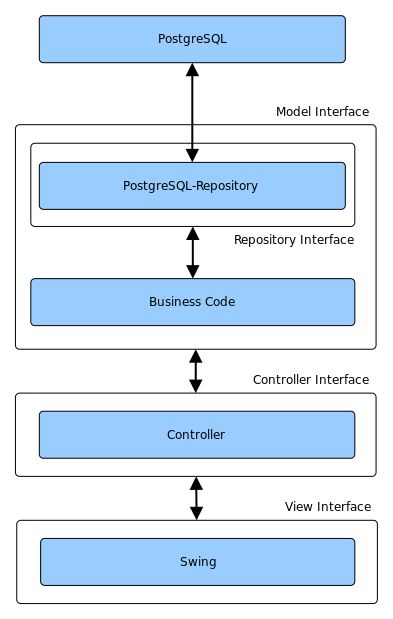
\includegraphics[width=0.4\textwidth]{./content/pictures/bpV1.jpg}
	\caption[Architectual Diagram of the best practice implementation in phase 1.]{Architectural Diagram of the best practice implementation in phase 1. All layers are 
	accessed using interfaces, the model layer accesses the databases through a separate data access layer in form of a repository interface.}
	\label{fig:bpV1}
\end{figure}

\begin{figure}[htbp]
		\centering
	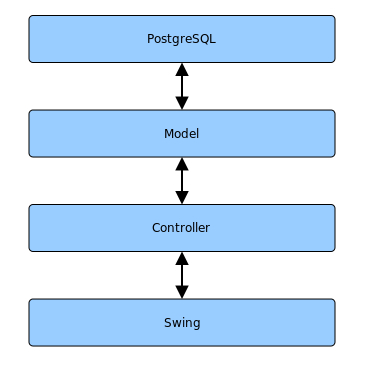
\includegraphics[width=0.4\textwidth]{./content/pictures/monoV1.jpg}
	\caption[Architectual Diagram of the ad-hoc implementation in phase 1.]{Architectural Diagram of the ad-hoc implementation in phase 1. No interfaces are used, all accesses are performed on concrete implementations.}
	\label{fig:monoV1}
\end{figure}



\subsection{Phase 2: Support of a different graphical user interface library}
After meeting the basic requirements the virtual stakeholders are requesting the support of a different GUI library, namely JavaFX (section \ref{sec:javafx}). By providing application start-up arguments the user should be able to decide which GUI should be presented to him. All other use-cases and requirements regarding the work flow apply nevertheless.

\subsection{Phase 3: Support of a different data tier implementation}
During the process the stakeholders request that the application should add support for MongoDB (section \ref{sec:mongodb}). They want to allow the user to choose between the two databases as both implementations have advantages and disadvantages. 

\begin{figure}[htbp]
		\centering
	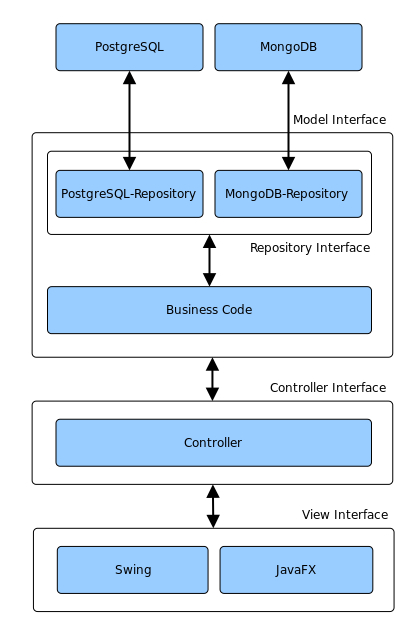
\includegraphics[width=0.5\textwidth]{./content/pictures/bpV3.jpg}
	\caption[Architectual Diagram of the best practice implementation in phase 3.]{Architectural Diagram of the best practice implementation in phase 3. As all layers are accessed using interfaces, the accesses of the model layer do not differ from phase 1. Only a new implementation of the repository interface needs to be added. The same situation occurs at the controller layer, where only a different view-interface implementation needs to be created.}
	\label{fig:bpV3}
\end{figure}

\begin{figure}[htbp]
		\centering
	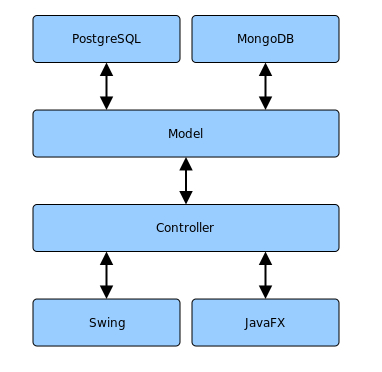
\includegraphics[width=0.5\textwidth]{./content/pictures/monoV3.jpg}
	\caption[Architectual Diagram of the ad-hoc implementation in phase 3.]{Architectural Diagram of the ad-hoc implementation in phase 3. As no interfaces are used, the model layer need to be able to access both the PostgreSQL and MongoDB database. The controller needs to access both the Swing and JavaFX view.}
	\label{fig:monoV3}
\end{figure}
%\subsection{Phase 4: Implementation of a cached controller}
%Several months after the deployment a customer reports performance issues and heavy load on their database server. Therefore it is decided to implement a caching algorithm for the controller to reduce expensive database calls. Again by starting the application with different arguments either the standard controller or the caching implementation should be used.

\clearpage
\section{Phase 1: Basic Requirements}
\label{sec:code-samples}
In the following sections the important parts of the applications implementations are shown and compared to each other in detail. As stated in the introduction the complete source code is available on Github. For more information on the project structure please refer to the appendix section.

\subsection{Best-Practice Code Samples}

\subsubsection{Database Access}
As an entry point for all data tier accesses, a class \texttt{DBManager} was created. It defines all available persistent storage options and is implemented as a singleton. The class itself is abstract, because each data access layer implementation needs to provide implementations for providing the repositories.
\begin{lstlisting}[caption={[DBManager singleton class.]DBManager singleton class. Used for instantiating the implementation of the chosen interface.}, captionpos=b, label={lst:dbmanager}]
public abstract class DBManager implements RepositoryFactory {
	private static final String DRIVER_POSTGRES = "org.postgresql.Driver";
	private static DBManager instance;
	
	public static synchronized DBManager get(String driver, String url, String username, String password) {
		switch(driver) {
		case DRIVER_POSTGRES:
			if(instance == null) instance = new DBManagerPostgres(driver, url, username, password);
			break;
		default:
			throw new UnsupportedOperationException("Not yet implemented");
		}
		return instance;
	}
}
\end{lstlisting}

The constructor of the PostgreSQL-database manager now initializes the connection based on the arguments provided. The interface \texttt{RepositoryFactory} is used to specify which methods each data access layer implementation has to override and which repositories there are. The overridden methods of the implementation invoke the constructor of the corresponding repository implementation and provides the data necessary for their work. In this case it is the Postgres-DBManager itself as it is often necessary for the repositories to load data by using other repositories.

\begin{lstlisting}[caption={Code snippet on how a DBManager implementation instantiates its repositories.}, captionpos=b]
public class DBManagerPostgres extends DBManager {
	...
	@Override
	public UserRepository getUserRepository() {
		return new UserRepositoryPostgres(this);
	}
	
	@Override
	public ProjectRepository getProjectRepository() {
		return new ProjectRepositoryPostgres(this);
	}
	...
}
\end{lstlisting}

In the business code it is now very easy to invoke the methods. The main model holds the only instance of the DBManager, each submodel has a reference to the main model. This process can be seen in listing \ref{lst:db-access-bp}.

\begin{lstlisting}[caption={[Code snippet showing how repositories are used in business code.]Code snippet showing how repositories are used in business code. The main model holds the single instance of the DBManager. Each sub-model accesses it by using a getter-method.}, captionpos=b, label={lst:db-access-bp}]
public void login(String username, char[] password) throws Exception {
	UserRepository repo = mainModel.db().getUserRepository();
	User u = repo.getByPrimaryKey(username);
	...
}
\end{lstlisting}

\subsubsection{UI Interaction}
As stated before there is a main controller that instantiates the sub-controllers. Because a pairing is necessary between model and controller the main controller provides methods to do so. After the main model has instantiated all sub-models they are paired with their associated controllers. This process is the implementation of \emph{dependency injection} as described in section \ref{sec:di}.

\begin{lstlisting}[caption={[Code snippet showing initialization code for the controller.]Code snippet showing initialization code for the controller. The main model retrieves the main controller by calling a getter which is similarily implemented as the DBManager class shown in listing \ref{lst:dbmanager}. After that he calls a method that pairs the sub-model with the sub-controller, a code snippet showing this process can be seen in listing \ref{lst:pairing}.}, captionpos=b, label={lst:db-manager-mono}]
private MainModelImpl(String driver, String url, String username, String password, String controllerImpl, String
frontend) throws Exception {
	db = DBManager.get(driver, url, username, password);
	ControllerManager.initInstance(controllerImpl, frontend);
	controller = ControllerManager.getInstance();
	controller.setModel(this);
	
	login = new LoginModelImpl();
	pairLogin();
	...
}

private void pairLogin() {
	login.setMainModel(this);
	controller.pairLogin(login);
}

\end{lstlisting}

The method call seen in line 4 of listing \ref{lst:db-manager-mono} states a call to the static ControllerManager class. Similar to the DBManager class this is a singleton class that holds a switch-case-statement that instantiates the main controller based on the implementation provided by the arguments. The method \texttt{pairLogin} shows how the sub-models are connected to their sub-controllers. 

\clearpage

The same process is repeated for the layer between controller and view. 

\begin{lstlisting}[caption={[Code snipped showing pairing code between a sub-controller and a sub-view.]Code snipped showing pairing code between a sub-controller and a sub-view. The pairing between the model and controller layer works in a very similar way.}, captionpos=b, label={lst:pairing}]
public class MainViewSwing {
	...
	public void pairLogin(LoginController controller) {
		controller.setView(login);
		login.setController(controller);
	}
	...
}
\end{lstlisting}
   
\subsection{Ad-hoc Code Samples}
In the first phase of the application not many differences can be observed. The advantages in flexibility introduced by the patterns shows its effect in the following phases. 

\subsubsection{Database Access}
As stated in section \ref{sec:ad-hoc} no repositories are used for the database access. All code associated with the persistent storage is directly placed into the data classes. They provide static methods for retrieve operations and non-static methods for update operations. 

As no interface is used the main model instantiates the DBManager implementation directly. 

\begin{lstlisting}[caption={[Code snipped showing database access in the ad-hoc program version. ]Code snipped showing database access in the ad-hoc program version. All database code is placed into the corresponding data class, retrieval methods are static and take the corresponding DBManager as parameter. The reference to the DBManager is provided by a getter method of the main model, as in listing \ref{lst:db-access-bp}.}, captionpos=b]
public void login(String username, char[] password) {
	User u = User.getByPrimaryKey(username, mainModel.db()); 
	...
}
\end{lstlisting}

\begin{lstlisting}[caption={[Code snippet showing how the DBManager is instantiated. ]Code snippet showing how the DBManager is instantiated. Again no interfaces but rather concrete implementations are used. The singleton class seen in listing \ref{lst:dbmanager} does not exist in the ad-hoc version.}, captionpos=b]
public class MainModelImpl {
	...
	private final DBManagerPostgres db;
	
	private MainModelImpl(String driver, String url, String username, String password, String controllerImpl, String
	frontend) throws Exception {
		db = new DBManagerPostgres(driver, url, username, password);
		...
	}
	...
}
\end{lstlisting}

\begin{lstlisting}[caption={[Code snippet showing a database access methods in a data class.]Code snippet showing a database access methods in a data class. The retrieval method takes arguments necessary for the query and the database-manager object as parameters and is static, while the update method is not static and therefore performs the operation on the current object instance.}, captionpos=b, label={lst:static-methods}]
public class User implements DBEntity {	
	...
	public static User getByPrimaryKey(String loginName, DBManagerPostgres db) throws Exception {
		...
	}
	
	public void insertIntoDb(DBManagerPostgres db) throws Exception {
		...
	}
	...
}
\end{lstlisting}

\subsubsection{UI Interaction}
The only difference between the pairing process of the best practice implementation and the ad-hoc version is that no interfaces are used and thus the methods take the implementation  classes instead of the interface as parameters. 
noticeable 
\begin{lstlisting}[caption={[Code snippet showing pairing code of the ad-hoc version of the program.]Code snippet showing pairing code of the ad-hoc version of the program. It is noticeable that the pairing method takes a concrete implementation rather than an interface as a parameter. This differs from the best practice version seen in \ref{lst:pairing} which takes only the interface as parameter.}, captionpos=b]
public class MainViewSwing {
	...
	public void pairLogin(LoginControllerStandard controller) {
		controller.setView(login);
		login.setController(controller);
	}
	...
}
\end{lstlisting}

\clearpage

\section{Phase 2: Support of a different graphical user interface library}
After adding the second GUI, clear differences between the two implementations can be observed.

\subsection{Best-Practice Code Samples}
Due to the use of the interfaces aside from implementing the view itself only very little modifications have to be made. Only the ViewManager-singleton class has to be adopted to support the new view \footnote{The internal structure of the JavaFX-Library needed the creation of a own thread. This is done by the calling \texttt{launchFx()}}.

\begin{lstlisting}[caption={View Manager after implementation of a second GUI. Only a case branch has to be added.}, captionpos=b]
public class ViewManager {
	private static MainView view;
	
	public static void initInstance(String frontend) {
		assert (view == null);
		switch(frontend) {
			case "standard":
				view = new MainViewSwing();
				break;
			case "javafx":
				MainViewFX fx = MainViewFX.getInstance();
				launchFx(fx);
				break;
			default:
				throw new UnsupportedOperationException();
		}
	}
	...
}
	
\end{lstlisting}

\subsection{Ad-hoc Code Samples}
\label{sec:ad-hoc-javafx}
Because the controllers do not rely on interfaces but upon actual implementations now each call to a view class has to be differentiated which bloats the code. The following if-else statement is necessary whenever a call to a view class is made. Obviously with more views the code is bloated even more, maybe then a switch-case would be used.

\begin{lstlisting}[caption={[Code snipped showing login-code after implementing a second GUI.]Code snipped showing login-code after implementing a second GUI. Because no interface but concrete implementations are used each time a view access is needed the program is required to check for which of the two GUIs is currently active. Controller methods of the best pratice version do not change in any way.}, captionpos=b, label={lst:controller-switch}]
public class LoginControllerStandard {
	private LoginViewSwing viewSwing;
	private LoginViewFX viewFX;
	...
	public void loginClicked() {
		String username;
		char[] password;
		if(viewSwing != null) {
			username = viewSwing.getEnteredUsername();
			password = viewSwing.getEnteredPassword();
		} else {
			username = viewFX.getEnteredUsername();
			password = viewFX.getEnteredPassword();
		}
		...
	}
	...
}
\end{lstlisting}

\clearpage
\section{Phase 3: Support of a different data tier implementation}
The support of a new data tier shows even more weaknesses of the ad-hoc implementation.

\subsection{Best-Practice Code Samples}
With the best-practice program version again only very small changes to existing code were necessary. Similar to phase 2 only the DBManager static method had to be adopted to support the other database.

\begin{lstlisting}[caption={DBManager implementation after support for a second database. Again only a branch of the switch-statement has to be added.}, captionpos=b]
public abstract class DBManager implements RepositoryFactory {
	private static final String DRIVER_POSTGRES = "org.postgresql.Driver";
	private static final String DRIVER_MONGO = "mongo";
	private static DBManager instance;
	
	public static DBManager get(String driver, String url, String username, String password) {
		switch(driver) {
			case DRIVER_POSTGRES:
				if(instance == null) instance = new DBManagerPostgres(driver, url, username, password);
				break;
			case DRIVER_MONGO:
				if(instance == null) instance = new DBManagerMongo(url, username, password);
				break;
			default:
			throw new UnsupportedOperationException("Not yet implemented");
		}
		return instance;
	}
}
\end{lstlisting}

\subsection{Ad-hoc Code Samples}
\label{sec:static-code-samples}
After changing all data classes to support the other data tier implementation all model classes needed to be adopted as well. This is because it had to be differentiated which database implementation is currently active. 

\begin{lstlisting}[caption={[Code of the login-process after implementing support of the second database in the ad-hoc version of the program. ]Code of the login-process after implementing support of the second database in the ad-hoc version of the program. Again because the application does not rely on interfaces as in listing \ref{lst:controller-switch} it has to be differentiated each time database access is needed. The methods for database code are overloaded.}, captionpos=b]
public class LoginModelImpl {
	...
	public void login(String username, char[] password) throws Exception {
		User u = null;
		if(mainModel.dbPostgres() != null)
			u = User.getByPrimaryKey(username, mainModel.dbPostgres());
		else
			u = User.getByPrimaryKey(username, mainModel.dbMongo());
		...
	}
	...
}
\end{lstlisting}